% ------------------------------------------------------------------------------
% TYPO3 CMS 7.3 - What's New - Chapter "Extbase & Fluid" (German Version)
%
% @author	Patrick Lobacher <patrick@lobacher.de> and Michael Schams <schams.net>
% @license	Creative Commons BY-NC-SA 3.0
% @link		http://typo3.org/download/release-notes/whats-new/
% @language	German
% ------------------------------------------------------------------------------
% LTXE-CHAPTER-UID:		ba9bf9d9-564d719b-a45c6394-358e2ef2
% LTXE-CHAPTER-NAME:	Chapter: Extbase & Fluid
% ------------------------------------------------------------------------------
% LTXE-SLIDE-START
% LTXE-SLIDE-UID:		b5ee213c-b04df592-d31ed084-b94e0f58
% LTXE-SLIDE-TITLE:		Feature #62242: ActionMenuItemGroupViewHelper (1)
% LTXE-SLIDE-REFERENCE:	Feature-62242-ActionMenuItemGroupViewHelper.rst
% ------------------------------------------------------------------------------

\begin{frame}[fragile]
	\frametitle{Extbase \& Fluid}
	\framesubtitle{ActionMenuItemGroupViewHelper (1)}

	% decrease font size for code listing
	\lstset{basicstyle=\tiny\ttfamily}

	\begin{itemize}

		\item Mit diesem neuen ViewHelper können im Backend Optionen-Gruppen für Select-Felder verwendet werden

		\item Beispiel:
			\begin{lstlisting}
				<f:be.menus.actionMenu>
				  <f:be.menus.actionMenuItem label="Default: Welcome" controller="Default" action="index" />
				  <f:be.menus.actionMenuItem label="Community: get in touch" controller="Community"
				    action="index" />
				  <f:be.menus.actionMenuItemGroup label="Information">
				    <f:be.menus.actionMenuItem label="PHP Information" controller="Information"
				      action="listPhpInfo" />
				    <f:be.menus.actionMenuItem label="Documentation" controller="Information"
				      action="documentation" />
				    <f:be.menus.actionMenuItem label="Hooks" controller="Information" action="hooks" />
				    <f:be.menus.actionMenuItem label="Signals" controller="Information" action="signals" />
				    <f:be.menus.actionMenuItem label="XClasses" controller="Information" action="xclass" />
				  </f:be.menus.actionMenuItemGroup>
				</f:be.menus.actionMenu>
			\end{lstlisting}

	\end{itemize}

\end{frame}

% ------------------------------------------------------------------------------
% LTXE-SLIDE-START
% LTXE-SLIDE-UID:		b04df592-d31ed084-b94e0f58-b5ee213c
% LTXE-SLIDE-TITLE:		Feature #62242: ActionMenuItemGroupViewHelper (2)
% LTXE-SLIDE-REFERENCE:	Feature-62242-ActionMenuItemGroupViewHelper.rst
% ------------------------------------------------------------------------------

\begin{frame}[fragile]
	\frametitle{Extbase \& Fluid}
	\framesubtitle{ActionMenuItemGroupViewHelper (2)}

	\begin{itemize}
		\item Beispiel auf der vorherigen Slide resultiert in folgender Ausgabe:
	\end{itemize}

	\begin{figure}
		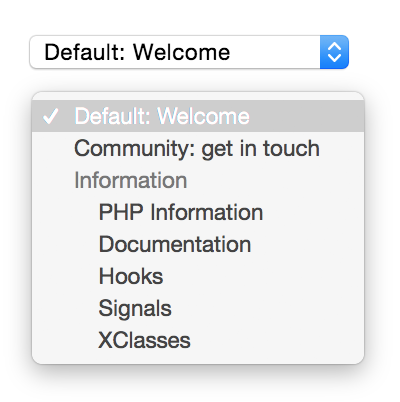
\includegraphics[width=0.3\linewidth]{ExtbaseFluid/62242.png}
	\end{figure}

\end{frame}

% ------------------------------------------------------------------------------
% LTXE-SLIDE-START
% LTXE-SLIDE-UID:		44467f9a-abe64946-3da2bf4c-5bd094eb
% LTXE-SLIDE-TITLE:		Feature: #63453 - Template support for FlashMessagesViewHelper
% LTXE-SLIDE-TITLE:		Breaking: #63453 - Changed rendering of FlashMessagesViewHelper
% LTXE-SLIDE-REFERENCE:	Feature-63453-TemplateSupportForFlashMessagesViewHelper.rst
% LTXE-SLIDE-REFERENCE:	Breaking-63453-ChangedRenderingOfFlashMessagesViewHelper.rst
% ------------------------------------------------------------------------------

\begin{frame}[fragile]
	\frametitle{Extbase \& Fluid}
	\framesubtitle{Template-Support für FlashMessagesViewHelper}

	% decrease font size for code listing
	\lstset{basicstyle=\tiny\ttfamily}

	\begin{itemize}

		\item Der \texttt{FlashMessagesViewHelper} hat nun Template Unterstützung

		\item Mit dem neuen Attribut \texttt{as} kann man eine Variable festlegen,
			über der der Zugriff auf die Messages möglich ist

		\item Beispiel:

			\begin{lstlisting}
				<f:flashMessages as="flashMessages">
				  <ul class="myFlashMessages">
				    <f:for each="{flashMessages}" as="flashMessage">
				      <li class="alert {flashMessage.class}">
				        <h4>{flashMessage.title}</h4>
				        <span class="fancy-icon">{flashMessage.message}</span>
				      </li>
				    </f:for>
				  </ul>
				</f:flashMessages>
			\end{lstlisting}

		\item Die Option \texttt{renderMode} ist ab sofort "deprecated"!

	\end{itemize}

\end{frame}

% ------------------------------------------------------------------------------
% LTXE-SLIDE-START
% LTXE-SLIDE-UID:		ec0810a7-c987f58a-9c42904e-8b7e0eba
% LTXE-SLIDE-TITLE:		Feature #66111: Add TemplateRootPaths support to cObject FLUIDTEMPLATE (1)
% LTXE-SLIDE-REFERENCE:	Feature-66111-AddTemplaterootpathsSupportToCobjectFluidtemplate.rst
% ------------------------------------------------------------------------------

\begin{frame}[fragile]
	\frametitle{Extbase \& Fluid}
	\framesubtitle{Neue Eigenschaften im cObject \texttt{FLUIDTEMPLATE} (1)}

	\begin{itemize}

		\item Das cObject \texttt{FLUIDTEMPLATE} wurde um die Eigenschaften
			\texttt{templateRootPaths} und \texttt{templateName} ergänzt

		\item Man kann nun einen Template-Namen setzen, der zusammen mit dem
			Format im angegebenen Template-Pfad gesucht wird

		\item \texttt{templateRootPaths} hat die selbe Fallback-Logik wie
			\texttt{layoutRootPath} und \texttt{partialRootPath}

			\begin{itemize}
				\item templateName (string/stdWrap)
				\item templateRootPaths (Array mit Datei-Pfaden und "EXT:" Unterstützung)
			\end{itemize}

	\end{itemize}

\end{frame}

% ------------------------------------------------------------------------------
% LTXE-SLIDE-START
% LTXE-SLIDE-UID:		ec0810a7-c987f58a-9c42904e-8b7e0eba
% LTXE-SLIDE-TITLE:		Feature #66111: Add TemplateRootPaths support to cObject FLUIDTEMPLATE (2)
% LTXE-SLIDE-REFERENCE:	Feature-66111-AddTemplaterootpathsSupportToCobjectFluidtemplate.rst
% ------------------------------------------------------------------------------

\begin{frame}[fragile]
	\frametitle{Extbase \& Fluid}
	\framesubtitle{Neue Eigenschaften im cObject \texttt{FLUIDTEMPLATE} (2)}

	% decrease font size for code listing
	\lstset{basicstyle=\tiny\ttfamily}

	\begin{itemize}

		\item TypoScript Beispiel:

			\begin{lstlisting}
				lib.stdContent = FLUIDTEMPLATE
				lib.stdContent {
				  templateName = TEXT
				  templateName.stdWrap {
				    cObject = TEXT
				    cObject {
				      data = levelfield:-2,backend_layout_next_level,slide
				      override.field = backend_layout
				      split {
				        token = frontend__
				        1.current = 1
				        1.wrap = |
				      }
				    }
				    ifEmpty = Default
				  }
				  templateRootPaths {
				    10 = EXT:frontend/Resources/Private/Templates
				    20 = EXT:sitemodification/Resources/Private/Templates
				  }
				}
			\end{lstlisting}

	\end{itemize}

\end{frame}


% ------------------------------------------------------------------------------
% LTXE-SLIDE-START
% LTXE-SLIDE-UID:		5d3c259c-f79dd1fe-4f272783-a63cf715
% LTXE-SLIDE-TITLE:		Feature #66269: Fluid: Remove ViewHelper xmlns-attributes and specified html tag (1)
% LTXE-SLIDE-REFERENCE:	Feature-66269-FluidRemoveViewHelperXmlnsAttributesAndSpecifiedHtmlTag.rst
% ------------------------------------------------------------------------------

\begin{frame}[fragile]
	\frametitle{Extbase \& Fluid}
	\framesubtitle{Entfernung von \texttt{xmlns}-Attributes und des HTML-Tags (1)}

	% decrease font size for code listing
	\lstset{basicstyle=\tiny\ttfamily}

	\begin{itemize}

		\item Durch die Einführung von \texttt{xmlns:*}-Attributen in Tags ist
			es einer IDE möglich Fluid direkt zu unterstützen
			(z.B. Syntax-Highlighting, Autovervollständigung, usw.).\newline
			Diese Attribute werden allerdings auch ausgegeben.

		\item Der Workaround, den eigentlichen Inhalt in Sections auszulagern,
			ist in Layouts nicht möglich und zudem nicht intuitiv

		\item Daher wird ein Namespace, sofern dieser den Aufbau
			\small\texttt{http://typo3.org/ns/<phpNamespace>}\space\normalsize
			hat, automatisch entfernt (alle anderen Namespaces bleiben erhalten)

	\end{itemize}

\end{frame}

% ------------------------------------------------------------------------------
% LTXE-SLIDE-START
% LTXE-SLIDE-UID:		27834f27-5d3c259c-f79dd1fe-a63cf715
% LTXE-SLIDE-TITLE:		Feature #66269: Fluid: Remove ViewHelper xmlns-attributes and specified html tag (2)
% LTXE-SLIDE-REFERENCE:	Feature-66269-FluidRemoveViewHelperXmlnsAttributesAndSpecifiedHtmlTag.rst
% ------------------------------------------------------------------------------

\begin{frame}[fragile]
	\frametitle{Extbase \& Fluid}
	\framesubtitle{Entfernung von \texttt{xmlns}-Attributes und des HTML-Tags (2)}

	% decrease font size for code listing
	\lstset{basicstyle=\tiny\ttfamily}

	\begin{itemize}

		\item Verwendet man im HTML-Tag das Attribut
			\texttt{data-namespace-typo3-fluid="true"}, wird das gesamte
			 HTML-Tag (öffnendes und schließendes) nicht gerendert

			\begin{lstlisting}
				<html data-namespace-typo3-fluid="true"
				  xmlns:f="http://typo3.org/ns/TYPO3/CMS/Fluid/ViewHelpers"
				  xmlns:n="http://typo3.org/ns/GeorgRinger/News/ViewHelpers">

				  <f:if condition="{newsItem.title}">
				    <f:then>
				      <n:titleTag>{newsItem.title}</n:titleTag>
				    </f:then>
				    <f:else>
				      <n:titleTag>News-Detail</n:titleTag>
				    </f:else>
				  </f:if>

				</html>
			\end{lstlisting}

	\end{itemize}

\end{frame}

% ------------------------------------------------------------------------------
% LTXE-SLIDE-START
% LTXE-SLIDE-UID:		f79dd1fe-4f272783-a63cf715-5d3c259c
% LTXE-SLIDE-TITLE:		Feature #66709: Add TemplateRootPaths support to Fluid/View/StandaloneView
% LTXE-SLIDE-REFERENCE:	Feature-66709-AddTemplateRootPathsSupportToFluidViewStandaloneView.rst
% ------------------------------------------------------------------------------

\begin{frame}[fragile]
	\frametitle{Extbase \& Fluid}
	\framesubtitle{Neue Methoden im Fluid-StandaloneView}

	% decrease font size for code listing
	\lstset{basicstyle=\tiny\ttfamily}

	\begin{itemize}

		\item Der StandaloneView wird mit den Methoden
			\texttt{setTemplateRootPaths(\$templatePaths)} und
			\texttt{setTemplate(\$templateName, \$throwException = TRUE)}
			erweitert

		\item Selbe Funktionalität wie im cObject \texttt{FLUIDTEMPLATE}

		\item Beispiel (Rendern eines Email-Templates):

			\begin{lstlisting}
				$view = GeneralUtility::makeInstance(StandaloneView::class);
				$view->setLayoutRootPaths(array(GeneralUtility::getFileAbsFileName(
				  'EXT:my_extension/Resources/Private/Layouts')));
				$view->setPartialRootPaths(array(GeneralUtility::getFileAbsFileName(
				  'EXT:my_extension/Resources/Private/Partials')));
				$view->setTemplateRootPaths(array(GeneralUtility::getFileAbsFileName(
				  'EXT:my_extension/Resources/Private/Templates')));
				$view->setTemplate('Email/Notification');
				$emailBody = $view->render();
			\end{lstlisting}

	\end{itemize}

\end{frame}

% ------------------------------------------------------------------------------
% LTXE-SLIDE-START
% LTXE-SLIDE-UID:		f79da63cf-7834f272-d1fe715-5d3c259c
% LTXE-SLIDE-TITLE:		Feature #66907: Add Data Processing to FLUIDTEMPLATE content object (1)
% LTXE-SLIDE-REFERENCE:	Feature-66907-AddDataProcessingToFluidTemplateContentObject.rst
% ------------------------------------------------------------------------------

\begin{frame}[fragile]
	\frametitle{Extbase \& Fluid}
	\framesubtitle{Data Processing für \texttt{FLUIDTEMPLATE} cObject (1)}

	% decrease font size for code listing
	\lstset{basicstyle=\smaller\ttfamily}

	\begin{itemize}

		\item Das cObject \texttt{FLUIDTEMPLATE} wird mit der Option
			\texttt{dataProcessing} (enthält ein Array aus FQCN) ausgerüstet,
			mit dessen Hilfe man das \texttt{\$data} Array manipulieren kann,
			welches das aktuell zu rendernde Objekt (wie \texttt{page} oder
			\texttt{tt\_content}) enthält

		\item Der Prozessor muss das Interface
			\texttt{FluidTemplateDataProcessorInterface} implementieren und
			folgende Methode enthalten:

			\begin{lstlisting}
				function process(array &$data, array $processorConfiguration,
				  array $configuration, StandaloneView $view) {
				    [...]
				}
			\end{lstlisting}

	\end{itemize}

\end{frame}

% ------------------------------------------------------------------------------
% LTXE-SLIDE-START
% LTXE-SLIDE-UID:		4f272783-a63cf715-5d3c259c-f79dd1fe
% LTXE-SLIDE-TITLE:		Feature #66907: Add Data Processing to FLUIDTEMPLATE content object (2)
% LTXE-SLIDE-REFERENCE:	Feature-66907-AddDataProcessingToFluidTemplateContentObject.rst
% ------------------------------------------------------------------------------

\begin{frame}[fragile]
	\frametitle{Extbase \& Fluid}
	\framesubtitle{Data Processing für \texttt{FLUIDTEMPLATE} cObject (2)}

	% decrease font size for code listing
	\lstset{basicstyle=\tiny\ttfamily}

	\begin{itemize}

		\item Beispiel:

			\begin{lstlisting}
				my_custom_ctype = FLUIDTEMPLATE
				my_custom_ctype {
				  templateRootPaths {
				    10 = EXT:your_extension_key/Resources/Private/Templates
				  }
				  templateName = CustomName
				  settings {
				    extraParam = 1
				  }
				  dataProcessing {
				    1 = Vendor\YourExtensionKey\DataProcessing\MyFirstCustomProcessor
				    2 = AnotherVendor\AnotherExtensionKey\DataProcessing\MySecondCustomProcessor
				    2 {
				      options {
				        myOption = SomeValue
				      }
				    }
				  }
				}
			\end{lstlisting}

	\end{itemize}

\end{frame}

% ------------------------------------------------------------------------------
